\documentclass{tcc}

\begin{document}
\setlength{\paperwidth}{21cm}
\setlength{\paperheight}{29.7cm}
\setlength{\pdfpagewidth}{\paperwidth}
\setlength{\pdfpageheight}{\paperheight}

\begin{center}
\Large{\bf \ ONLINE RETAIL MANAGEMENT SYSTEM}\\
\end{center}

\begin{center}
\ BY\\
\end{center}

\begin{center}
\ AISHWARYA SRINIVASAN\hspace{1.3cm} - 13BCE1006\\
\ SHASHANK DEVISETTY\hspace{1.5cm}    - 13BCE1036\\
\ HARSHWARDHAN AGARWAL\hspace{0.5cm} - 13BCE1052\\
\ SHASHANK M V \hspace{3cm}  - 13BCE1081\\
\end{center}
\ \\

\begin{center}
\textit{A project submitted to the}\\
\textbf{SCHOOL OF COMPUTING SCIENCES AND ENGINEERING}\\
\textit{in partial fulfillment of the award for the degree}\\
\textit{of}\\
\textbf{BACHELOR OF TECHNOLOGY}\\
\textit{in}\\
\textbf{COMPUTER SCIENCE ENGINEERING}\\
\end{center}
\ \\
\begin{figure}[H]
\centering

\includegraphics{images/vit.png}\\
VELLORE INSTITUTE OF\\ TECHNOLOGY\\
CHENNAI CAMPUS\\
NOV, \the\year
\end{figure}

\newpage
\begin{center}
\textbf{ACKNOWLEDGEMENT}\\
\end{center}
\begin{flushleft}
Course Code: CSE328 \hspace{1.4cm} Course Title: SOFTWARE PROJECT MANAGEMENT\\
\end{flushleft}
This project report entitled \textbf{“ONLINE RETAIL MANAGEMENT SYSTEM”} is a bonafide work of \textbf{AISHWARYA SRINIVASAN (13BCE1006), SHASHANK. D (13BCE1036), HARSHWARDHAN AGARWAL (13BCE1052) and SHASHANK. M. V (13BCE1081)} and had been carried out under the supervision and guidance of \textbf{Prof. Aparna. V}. We wish to express our sincere thanks and deep sense of gratitude to our project guide, \textbf{Prof. Aparna. V}, Assistant Professor, School of Computing Sciences and Engineering for her consistent encouragement and valuable guidance offered to us in a pleasant manner throughout the course of the project work.\\
\vspace{0.2in}
\vfill
\begin{flushleft}
\textbf{SHASHANK. D \hspace{5.4cm} HARSHWARDHAN AGARWAL}\\
\textbf{SHASHANK. M. V \hspace{4.6cm} AISHWARYA SRINIVASAN}
\end{flushleft}

\newpage
\begin{center}
\textbf{\Large{ABSTRACT}}
\end{center}
\vspace{0.1in}
Online Retail Management Software is a software application to be developed for the use in any retail unit/shop. The software aims at computerizing all the activities related to the retail unit. It should be a comprehensive one to cover all the aspects of a retail shop.

\begin{center}
\textbf{\Large{INTRODUCTION}}
\end{center}
\vspace{0.1in}
Online Retail Management System is a form of electronic shopping store where the buyer interacts directly with the seller usually via the internet. There is no intermediary service. The sale and purchase transaction is completed electronically and interactively in real-time. The development of this new system contains the following activities, which try to develop on-line application by keeping the entire process in the view of database integration approach.\\
\\
\textbf{Administrator} of Online Retail Management System has multiple features such as Add,Delete, Update shopping Items.\\
\\
\textbf{Customer} of Online Retail Management System has multiple features such as Sign up,Login, Shop online, Get an invoice.\\
\\
\textbf{\underline{Features of Online Retail Management System:}}\\
\\
1.	Secure registration and profile management facilities for Customers. \\
\\
2.	Browsing through the e-Mall to see the items that are there in each category of products like Apparel, Kitchen accessories, Bath accessories, Food items etc.\\ 
\\
3.	Creating a Shopping cart so that customer can Shop N number of items and checkout finally with the entire shopping cart\\
\\
4.	Customers should be able to mail the Shop about the items they would like to see in the Shop\\ 
\\
5.	Secured mechanism for checking out from the Shop ( Credit card verification mechanism ). Updates to customers about the Recent Items in the Shop.\\ 
\\
\newpage
\begin{flushleft}
6.	Uploading Most Purchased Items in each category of products in the Shop like Apparel, Kitchen accessories, Bath accessories, Food items etc.\\
\end{flushleft}
\begin{center}
\textbf{\Large{ER DIAGRAM}}
\end{center}
\begin{figure}[H]
\centering
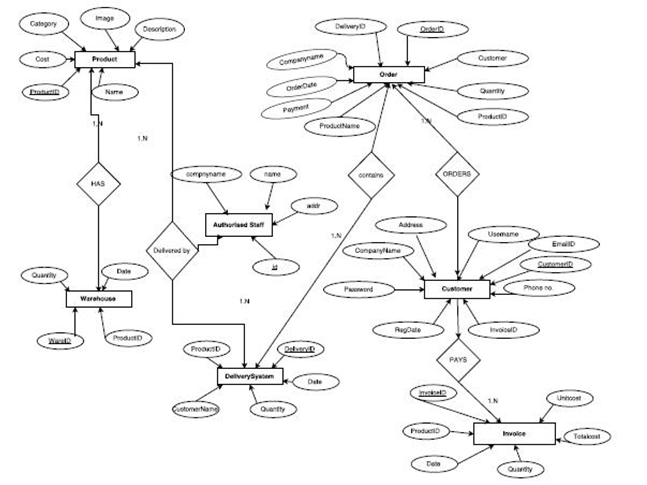
\includegraphics{images/er.PNG}\\
\end{figure}

\begin{center}
\textbf{\Large{MODULES}}
\end{center}
Our project consists of several modules namely,
\begin{itemize}
    \item Administrator
    \begin{itemize}
        \item Add a product
        \item Modify a product
        \item Delete a product
        \item Search a product
    \end{itemize}
    \newpage
    \item Customer
    \begin{itemize}
        \item Login
        \item Sign up
        \item Shop products
        \item Generate Invoice
    \end{itemize}
\end{itemize}
\begin{center}
\textbf{\Large{SQL}}
\end{center}
SQL stands for Structured Query Language. SQL is used to communicate with a database. According to ANSI (American National Standards Institute), it is the standard language for relational database management systems. SQL statements are used to perform tasks such as update data on a database, or retrieve data from a database. Some common relational database management systems that use SQL are: Oracle, Sybase, Microsoft SQL Server, Access, Ingres, etc. Although most database systems use SQL, most of them also have their own additional proprietary extensions that are usually only used on their system. However, the standard SQL commands such as "Select", "Insert", "Update", "Delete", "Create", and "Drop" can be used to accomplish almost everything that one needs to do with a database. This tutorial will provide you with the instruction on the basics of each of these commands as well as allow you to put them to practice using the SQL Interpreter.
\begin{center}
\textbf{\Large{ESTABLISHING CONNECTION WITH DATABASE}}
\end{center}
\begin{figure}[H]
\centering
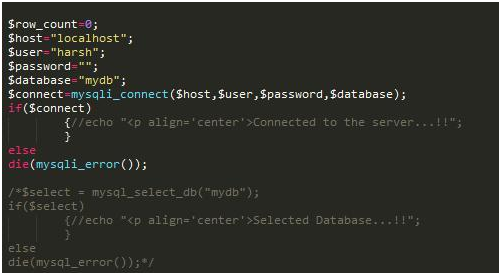
\includegraphics{images/1.PNG}\\
\end{figure}

\newpage
\begin{flushleft}
\Large{{\fontfamily{ptm}\selectfont
Administrator:
}}
\end{flushleft}

\begin{enumerate}
    \item Add a product
    \begin{figure}[H]
    \centering
    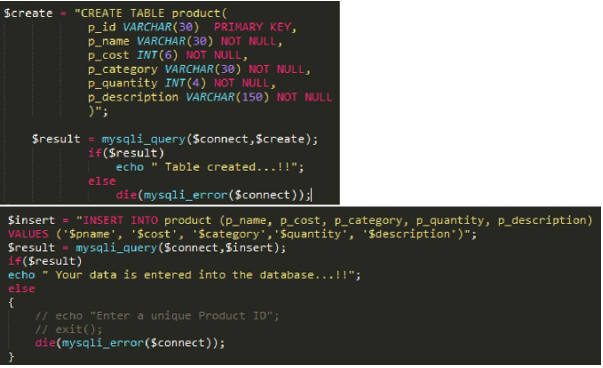
\includegraphics{images/2.PNG}\\
    \end{figure}
    \item Modify a Product
    \begin{figure}[H]
    \centering
    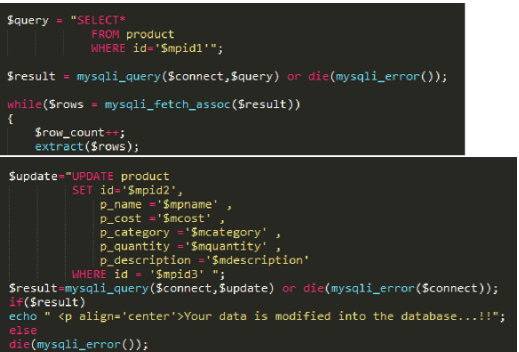
\includegraphics{images/3.PNG}\\
    \end{figure}
    \ \\
    \item Delete a Product
    \begin{figure}[H]
    \centering
    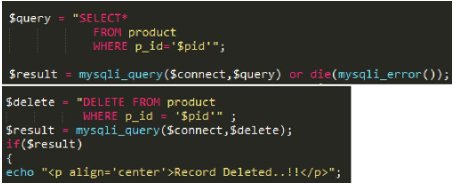
\includegraphics{images/4.PNG}\\
    \end{figure}
    \item Search a Product
    \begin{figure}[H]
    \centering
    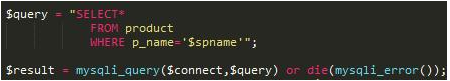
\includegraphics{images/5.PNG}\\
    \end{figure}
\end{enumerate}
\begin{flushleft}
\Large{{\fontfamily{ptm}\selectfont
Customers:
}}
\end{flushleft}

\begin{enumerate}
    \item Sign Up
    \begin{figure}[H]
    \centering
    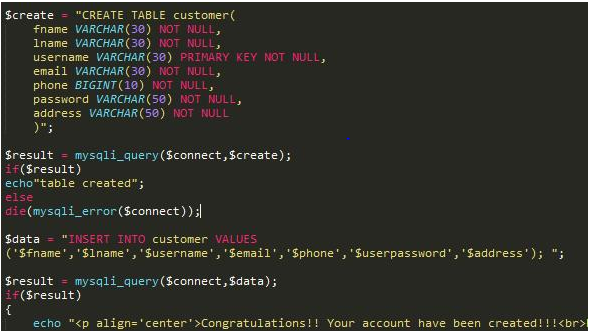
\includegraphics{images/6.PNG}\\
    \end{figure}
    \item Login
    \begin{figure}[H]
    \centering
    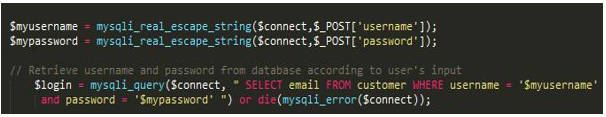
\includegraphics{images/7.PNG}\\
    \end{figure}
    \ \\
    \item Shop Products
    \begin{figure}[H]
    \centering
    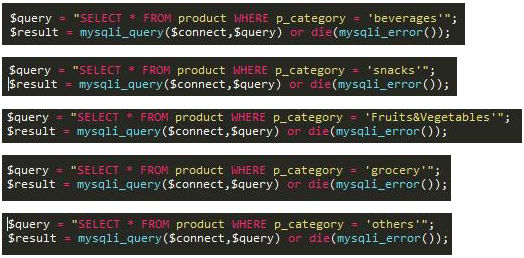
\includegraphics{images/8.PNG}\\
    \end{figure}
    Also \textbf{“Recommendations”} have been provided based on the past purchases of a particular customer and also based on table-mapping i.e. for example, if a customer buys shoes, the portal would recommend socks for him/her.
    \begin{figure}[H]
    \centering
    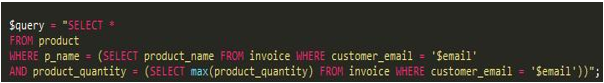
\includegraphics{images/9.PNG}\\
    \end{figure}
    \newpage
    \item Generate an invoice\\
    \begin{figure}[H]
    \centering
    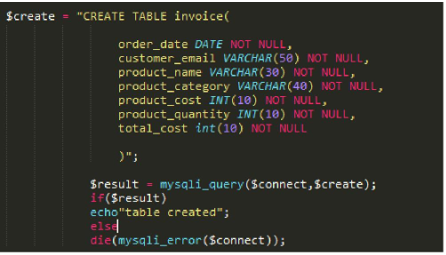
\includegraphics{images/10.PNG}\\
    \end{figure}
    \begin{figure}[H]
    \centering
    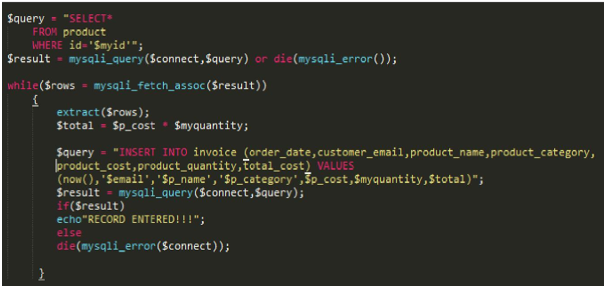
\includegraphics{images/11.PNG}\\
    \end{figure}
\end{enumerate}
\newpage
\begin{center}
\textbf{\Large{USECASE DIAGRAM}}
\end{center}
\begin{figure}[H]
\centering
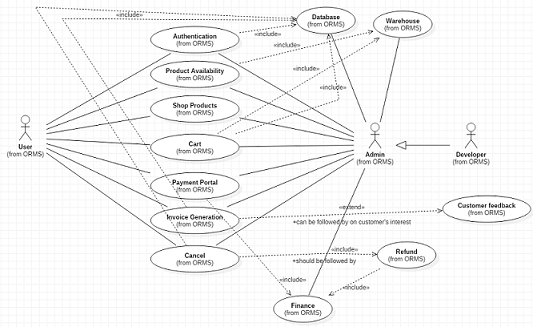
\includegraphics{images/usecase.png}\\
\end{figure}
\begin{center}
\textbf{\Large{SUB-USECASE DIAGRAMS}}
\end{center}
\begin{flushleft}
\Large{{\fontfamily{ptm}\selectfont
Authentication:
}}
\end{flushleft}
\begin{figure}[H]
\centering
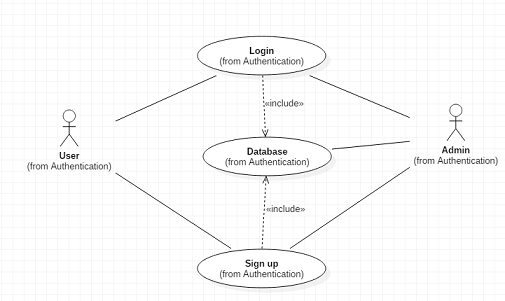
\includegraphics{images/authentication.PNG}\\
\end{figure}
\ \\ \\
\begin{flushleft}
\Large{{\fontfamily{ptm}\selectfont
Product Availability:
}}
\end{flushleft}
\begin{figure}[H]
\centering
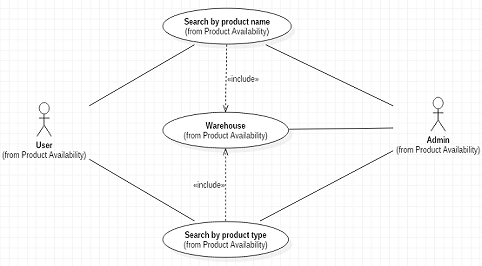
\includegraphics{images/productavailability.PNG}\\
\end{figure}
\begin{flushleft}
\Large{{\fontfamily{ptm}\selectfont
Shop Products:
}}
\end{flushleft}
\begin{figure}[H]
\centering
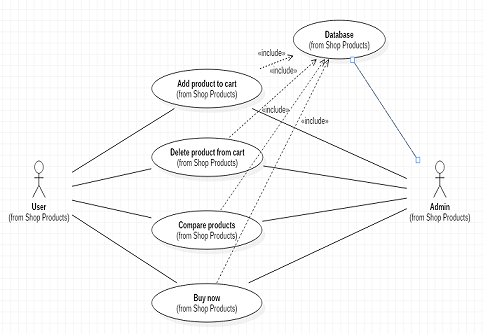
\includegraphics{images/shopproducts.PNG}\\
\end{figure}
\ \\ \\ \\ \\ \\
\begin{flushleft}
\Large{{\fontfamily{ptm}\selectfont
Cart:
}}
\end{flushleft}
\begin{figure}[H]
\centering
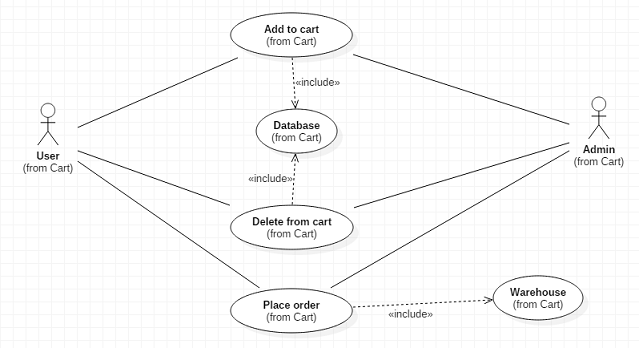
\includegraphics{images/cart.PNG}\\
\end{figure}
\begin{flushleft}
\Large{{\fontfamily{ptm}\selectfont
Payment Portal:
}}
\end{flushleft}
\begin{figure}[H]
\centering
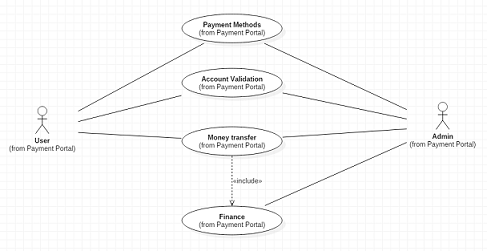
\includegraphics{images/paymentportal.PNG}\\
\end{figure}
\newpage
\begin{flushleft}
\Large{{\fontfamily{ptm}\selectfont
Invoice Generation:
}}
\end{flushleft}
\begin{figure}[H]
\centering
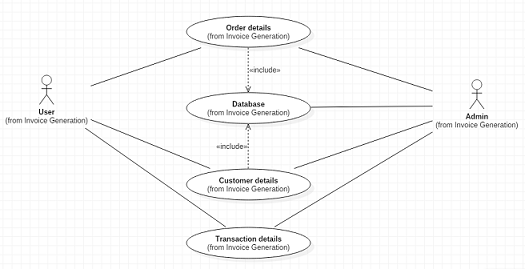
\includegraphics{images/invoicegeneration.PNG}\\
\end{figure}
\begin{flushleft}
\Large{{\fontfamily{ptm}\selectfont
Cancel:
}}
\end{flushleft}
\begin{figure}[H]
\centering
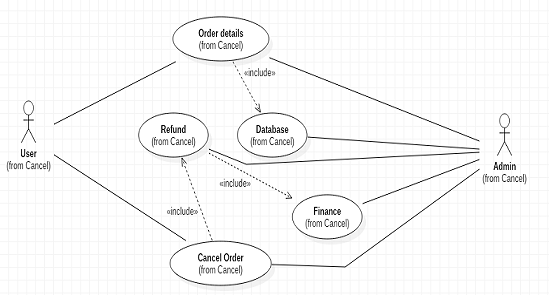
\includegraphics{images/cancel.PNG}\\
\end{figure}
\newpage
\begin{center}
\textbf{\Large{SEQUENCE DIAGRAMS}}
\end{center}
\begin{figure}[H]
\centering
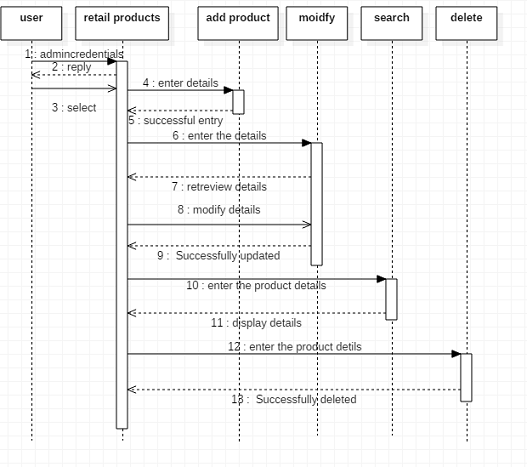
\includegraphics{images/prductmodifyseq1.PNG}\\
\end{figure}
\begin{figure}[H]
\centering
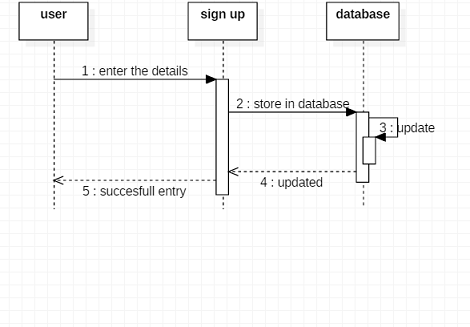
\includegraphics{images/signup.PNG}\\
\end{figure}
\begin{figure}[H]
\centering
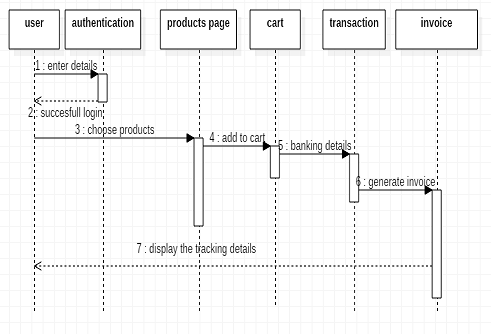
\includegraphics{images/addingtocartseq.PNG}\\
\end{figure}
\begin{center}
\textbf{\Large{OUTCOME}}
\end{center}
\begin{center}
\textbf{\Large{HOMEPAGE}}
\end{center}
\begin{figure}[H]
\centering
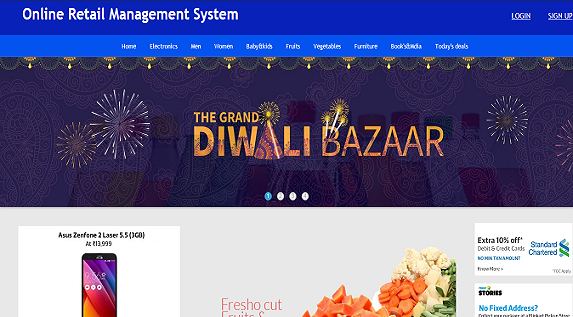
\includegraphics{images/sc1.PNG}\\
\end{figure}
\newpage
\begin{center}
\textbf{\Large{SIGN IN}}
\end{center}
\begin{figure}[H]
\centering
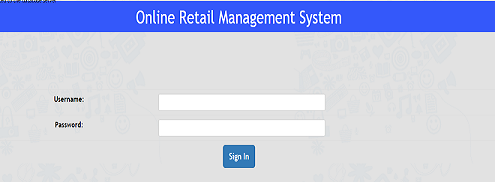
\includegraphics{images/sc2.PNG}\\
\end{figure}
\begin{center}
\textbf{\Large{ORDERING}}
\end{center}
\begin{figure}[H]
\centering
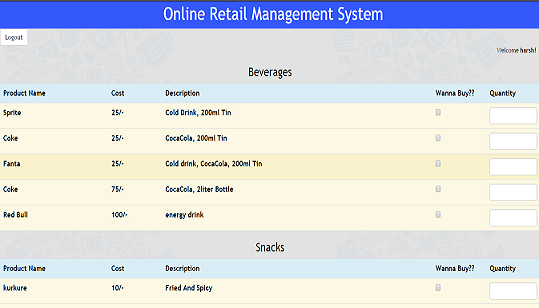
\includegraphics{images/sc3.PNG}\\
\end{figure}
\newpage
\begin{center}
\textbf{\Large{RECOMMENDATIONS}}
\end{center}
\begin{figure}[H]
\centering
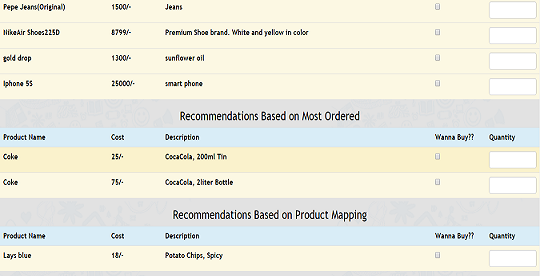
\includegraphics{images/sc4.PNG}\\
\end{figure}
\begin{center}
\textbf{\Large{SPM Techniques in ORMS}}
\end{center}
\begin{flushleft}
\Large{{\fontfamily{ptm}\selectfont
Recommendations:
}}
\end{flushleft}
The goal of a Recommender System is to generate meaningful recommendations to a collection of users for items or products that might interest them.  The design of such recommendation engines depends on the domain and the particular characteristics of the
data available.Such a data source records the quality of interactions between users and items. Additionally, the system may have access to user-specific and item-specific profile attributes such as demographics and product descriptions respectively. Recommender systems differ in the way they analyze these data sources to develop notions of affinity between users and items which can be used to identify well-matched pairs.
The myriad approaches to Recommender Systems can be broadly categorized as
\begin{enumerate}
    \item Collaborative Filtering (CF): In CF systems a user is recommended items based on the past ratings of all users collectively.
    \item Content-based recommending: These approaches recommend items that are similar in content to items the user has liked in the past, or matched to attributes of the user.
    \item Hybrid approaches: These methods combine both collaborative and content based approaches.
\end{enumerate}
\newpage
\begin{flushleft}
\Large{{\fontfamily{ptm}\selectfont
Collaborative Filtering:
}}
\end{flushleft}
Collaborative filtering is most extensively used approach to design recommender system. Collaborative Filtering (CF) methods play an significant role in the recommendation process, although Collaborative filtering is often used along with other filtering techniques like content-based, knowledge based. Basically Collaborative filtering methods are established on gathering and examining a large amount of information which based on users demeanor, activities or preferences and anticipating taste of that particular user by
using their similarity with other users. It does not depend on machine decomposable message and thus it is correctly recommending composite items and because of that it is a key benefit of the collaborative filtering approach. In collaborative filtering recommendation system recommended objects are selected on the basis of past evaluations of a large group of users.
\begin{flushleft}
Advantages:
\end{flushleft}
\begin{enumerate}
    \item Memory-Based Collaborative filtering techniques makes implementation of recommendation system easier.
    \item Using Memory-Based Collaborative filtering techniques one can add new data easily and in incremental manner.
    \item Model-Based Collaborative filtering techniques improves prediction performance.
\end{enumerate}
\begin{flushleft}
Disadvantages:
\end{flushleft}
\begin{enumerate}
    \item Cold Start: CF systems often require a huge amount of existing data on which user can make exact recommendations.
    \item Scalability: CF makes recommendations for various environments where billions of users and products exist. Therefore, a huge amount of computation power is often essential to compute recommendations.
    \item Sparsity: On major e-commerce site the number of items sold are enormously large. Because of that only a small subset of the entire database is rated by most active users. Hence very few ratings are given to the most popular items.
\end{enumerate}
\newpage
\begin{flushleft}
\Large{{\fontfamily{ptm}\selectfont
Content Based Filtering:
}}
\end{flushleft}
Content-based filtering (CBF) tries to recommend items to the active user based on similarity count which is rated by that user positively in the past.
\begin{flushleft}
Advantages:
\end{flushleft}
\begin{enumerate}
    \item Content-based recommender system provide user independence through exclusive ratings which are used by the active user to build their own profile.
    \item Content-based recommender system provide Transparency to their active user by giving explanation how recommender system works.
    \item Content-based recommenders system are adequate to recommend items not yet placed by any user. This will be advantageous for new user.
\end{enumerate}
\begin{flushleft}
Disadvantages:
\end{flushleft}
\begin{enumerate}
    \item It is a difficult task to generate the attributes for items in certain areas.
    \item CBF advocate the same types of items because of that it suffers from an overspecialization problem.
    \item It is harder to acquire feedback from users in CBF because users do not typically rank the items (as in CF) and therefore, it is not possible to determine whether the recommendation is correct.
\end{enumerate}
\begin{flushleft}
\Large{{\fontfamily{ptm}\selectfont
Conclusion:
}}
\end{flushleft}
Classic Collaborative Filtering was proven to be the best performing algorithm. The smart non-personalized approach performed surprising well. Item-based Filtering displayed disappointing behavior. Collaborative Filtering algorithm focuses on similar users as judged by their ratings, collecting them in user neighborhoods, whereas Item-based Filtering focuses on similar items as judged by user ratings, collecting them in item neighborhoods.
\end{document}